%ドキュメントクラスの指定。使えるならばjsarticleを指定し、
% そうでなければjarticleを指定する。しかしjsarticleがない環境は
% 新しい環境に更新すべきだと思う。
%   - 10pt:       本文の文字サイズを10ptにする。実用上は10ptか11ptを指定する。
%   - a4j:        用紙サイズを日本語用A4サイズにする。
%                 報告書は日本語なので必要。
%   - twocolumn:  二段組にする。
%                 報告書のフォーマットは二段組なので基本的に必要。
%   - dvipdfmx:   画像の描画にdvipdfmxを使う。
%                 後述のgraphicxパッケージを使うときに必要。
%   - uplatex:    TeXの処理系をupLaTeXにする。
%                 **処理系がpLaTeXのときは 削 除 すること。**
\documentclass[10pt, a4j, uplatex, dvipdfmx, twocolumn]{jsarticle}


\usepackage{graphicx}   % \includegraphics を使うためのパッケージ読み込み
\usepackage{imcreport,bm,amsmath,amssymb}  % IMC報告会用テンプレートパッケージの読み込み


% ハイフネーションを抑制する。数値が大きいほど、無理にでも抑制しようとする。
\hyphenpenalty=10000\relax
\exhyphenpenalty=10000\relax
\sloppy


\title{ロボットアームを搭載した宇宙機の姿勢制御}%Hamilton-Jacobi方程式の近似計算法   % タイトル
\author{久門田 諒}                                % 著者
\studentnumber{TM21K020}                        % 学籍番号
\date{2021年11月22日}                            % 日付
\header{後期中間報告}                 % 左上のヘッダ内容

% 報告会で使われるフォーマットに従った\pLaTeX(またはu\pLaTeX)のテンプレート,``imcreport.sty''を作りました.この資料では作成したフォーマットを使ったサンプルの提示と,テンプレートの使い方の説明をします.
% この資料では\pLaTeX のクラスは``jsarticle''を指定していることを前提にしています。資料によってはjarticleを使っていることもありますが、jarticleよりもjsarticleのほうがきれいに組版されるので使える環境ではjsarticleを使うようにしましょう。

\begin{document}

\maketitle

\section{はじめに}
宇宙ロボットは故障衛星の修理,デブリの除去などの用途に使用されている.
宇宙空間での作業では,地球上と違い,ロボットアームの運動の反作用で宇宙ロボット本体の姿勢が変化する,
ターゲットが回転している,故障衛星など質量の大きいターゲットを把持した場合,宇宙ロボットのパラメータが変化するなどの特徴がある.
% また,ターゲットを捕獲する手順としてロボットアームのターゲット把持部へ接近,把持,把持によって質量パラメータが変化した宇宙ロボットの姿勢,ロボットアームの制御がある.
本報告書では,ターゲットの把持,その後,質量パラメータが変化した宇宙ロボットのロボットアーム,姿勢の速度を0にするため,
スライディングモード制御を絶対上界値を与える方法\cite{nonami}を検討した.
\section{宇宙ロボットのモデル}
宇宙ロボットのモデルを図\ref{space}に示す.リンクの長さを$l_i$($i=0,1,2,3$),
宇宙ロボット本体の位置を$X,Y$,宇宙ロボットの姿勢,関節角度を$\theta_i$($i=0,1,2,3$)とする.
\section{運動方程式}
宇宙ロボットの運動方程式はラグランジュの運動方程式から求める.
ここで,$\bm{M}(\bm{\theta})$は慣性行列,$\bm{h}(\bm{\theta},\dot{\bm{\theta}})$は遠心力,コリオリ力などをまとめたものであり,
$\bm{u}(t)$は宇宙ロボットの並進制御力ベクトル,姿勢制御および関節トルク入力ベクトルである.
\begin{equation}
    \bm{M}(\bm{\theta})\ddot{\bm{q}}(t)+\bm{h}(\bm{\theta},\dot{\bm{\theta}})=\bm{u}(t)
\end{equation}
また,
\begin{align*}
    \bm{q}=&
    \begin{bmatrix}
        X&Y&\theta_0&\theta_1&\theta_2&\theta_3
    \end{bmatrix}^T\\
    \bm{\theta}=&
    \begin{bmatrix}
        \theta_0&\theta_1&\theta_2&\theta_3
    \end{bmatrix}^T
\end{align*}
さらに,
\begin{equation}
    \bm{M}(\bm{\theta})=\bm{M}^0(\bm{\theta})+\Delta\bm{M}(\bm{\theta})
\end{equation}
\begin{equation}
    \bm{h}(\bm{\theta},\dot{\bm{\theta}})=\bm{h}^0(\bm{\theta},\dot{\bm{\theta}})+\Delta\bm{h}(\bm{\theta},\dot{\bm{\theta}})
\end{equation}
とし,
$\bm{M}(\bm{\theta})$,$\bm{h}(\bm{\theta},\dot{\bm{\theta}})$を公称値,$\Delta\bm{M}(\bm{\theta})$,$\Delta\bm{h}(\bm{\theta},\dot{\bm{\theta}})$
を実際値からの誤差とする.
ここで,$\Delta\bm{M}(\bm{\theta})$,$\Delta\bm{h}(\bm{\theta},\dot{\bm{\theta}})$,
$\bm{M}(\bm{\theta})$の時間微分値$\dot{\bm{M}}_{ij}(\bm{\theta})$の要素の絶対上界値を以下のように定義する.
\begin{align}
    |\Delta\bm{M}_{ij}(\bm{\theta})|&\leq \hat{\bm{M}}_{ij}(\bm{\theta})\\
    |\Delta\bm{h}_i(\bm{\theta},\dot{\bm{\theta}})|&\leq \hat{\bm{h}}_i(\bm{\theta},\dot{\bm{\theta}})\\
    |\dot{\bm{M}}_{ij}(\bm{\theta})|&\leq \hat{\dot{\bm{M}}}_{ij}(\bm{\theta})
\end{align}
また,絶対上界値$\hat{v}_i(\bm{\theta},t)$を以下のようにおく.
\begin{equation}
    |\{\bm{M}(\bm{\theta})\ddot{\bm{q}}_d(t)\}_i|\leq \hat{v}_i(\bm{\theta},t)
\end{equation}

\section{制御方法}
まず,切換超平面を設計する.目標軌道$\bm{q}_d$とし,追従誤差を以下のようにする.
\begin{align}
    \bm{e}(t)=\bm{q}(t)-\bm{q}_d(t)\\
    \dot{\bm{e}(t)}=\dot{\bm{q}}(t)-\dot{\bm{q}}_d(t)
\end{align}
上記の式を用いて,次のように切換超平面を設計する.
\begin{equation}
    \bm{\sigma}(t)=\bm{\Lambda}\bm{e}(t)+\dot{\bm{e}}(t)
\end{equation}
ここで,
\begin{equation*}
    \bm{\Lambda}=diag(\lambda_1,\cdots,\lambda_n),\ \ \ \lambda_i >0
\end{equation*}
とする.$\bm{\sigma}(t)=0$が成立すれば,$\bm{e}(\infty)\rightarrow 0$が保障される.
状態が初期値から超平面へ到達することを保障するために,
次のようなリアプノフ関数を用いて安定となるように入力を決定する.
\begin{equation}
    V(\sigma)=\frac{1}{2}\bm{\sigma}^T\bm{M}\bm{\sigma}
\end{equation}
\begin{equation}
    \bm{u}(t)=-\bm{M}^0(\bm{\theta})\bm{\Lambda}\dot{\bm{e}}(t)+\bm{h}^0(\bm{\theta},\dot{\bm{\theta}})-\bm{P\sigma}-\bm{Q}sgn(\bm{\sigma})
\end{equation}
ここで,行列$\bm{P},\bm{Q}$は対角行列である.
\begin{figure}[t]
    \centering
    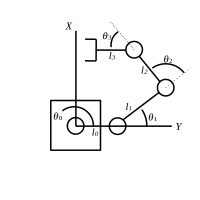
\includegraphics[width=50mm]{space_robot_model.pdf}
    \caption{宇宙ロボットのモデル}
    \label{space}
\end{figure}


\begin{thebibliography}{9}
\bibitem{nonami}野波健蔵,田宏奇,スライディングモード制御ー非線形ロバスト制御の設計理論ー,コロナ社(1994)
\bibitem{tuda}小林拓郎,津田慎一,宇宙ロボットによるターゲット捕獲のための制御,第53回自動制御連合講演会,pp.940-944(2010)
\end{thebibliography}

\end{document}